

\documentclass[conference]{IEEEtran}
%\documentclass[conference]{IEEEconf_allowlinks}




% *** CITATION PACKAGES ***
%
\usepackage{cite}
\usepackage{listings} % FOR CODE BLOCK 



% NOTE: %% from wikibooks

\usepackage{color}

\definecolor{mygreen}{rgb}{0,0.6,0}
\definecolor{mygray}{rgb}{0.5,0.5,0.5}
\definecolor{mymauve}{rgb}{0.58,0,0.82}

\lstset{
  backgroundcolor=\color{white},   % choose the background color; you must add \usepackage{color} or \usepackage{xcolor}; should come as last argument
  basicstyle=\footnotesize,        % the size of the fonts that are used for the code
  breakatwhitespace=false,         % sets if automatic breaks should only happen at whitespace
  breaklines=true,                 % sets automatic line breaking
  captionpos=b,                    % sets the caption-position to bottom
  commentstyle=\color{mygreen},    % comment style
  deletekeywords={...},            % if you want to delete keywords from the given language
  escapeinside={\%*}{*)},          % if you want to add LaTeX within your code
  extendedchars=true,              % lets you use non-ASCII characters; for 8-bits encodings only, does not work with UTF-8
  firstnumber=1000,                % start line enumeration with line 1000
  frame=single,                    % adds a frame around the code
  keepspaces=true,                 % keeps spaces in text, useful for keeping indentation of code (possibly needs columns=flexible)
  keywordstyle=\color{blue},       % keyword style
  language=Octave,                 % the language of the code
  morekeywords={*,...},            % if you want to add more keywords to the set
  %numbers=left,                    % where to put the line-numbers; possible values are (none, left, right)
  %numbersep=5pt,                   % how far the line-numbers are from the code
  %numberstyle=\tiny\color{mygray}, % the style that is used for the line-numbers
  rulecolor=\color{black},         % if not set, the frame-color may be changed on line-breaks within not-black text (e.g. comments (green here))
  showspaces=false,                % show spaces everywhere adding particular underscores; it overrides 'showstringspaces'
  showstringspaces=false,          % underline spaces within strings only
  showtabs=false,                  % show tabs within strings adding particular underscores
  stepnumber=2,                    % the step between two line-numbers. If it's 1, each line will be numbered
  stringstyle=\color{mymauve},     % string literal style
  tabsize=2,                     % sets default tabsize to 2 spaces
  title=\lstname                   % show the filename of files included with \lstinputlisting; also try caption instead of title
}
\usepackage{hyperref}


% *** GRAPHICS RELATED PACKAGES ***
%
\ifCLASSINFOpdf
   \usepackage[pdftex]{graphicx}
  % declare the path(s) where your graphic files are
  % \graphicspath{{../pdf/}{../jpeg/}}
  % and their extensions so you won't have to specify these with
  % every instance of \includegraphics
  % \DeclareGraphicsExtensions{.pdf,.jpeg,.png}
\else
  % or other class option (dvipsone, dvipdf, if not using dvips). graphicx
  % will default to the driver specified in the system graphics.cfg if no
  % driver is specified.
  % \usepackage[dvips]{graphicx}
  % declare the path(s) where your graphic files are
  % \graphicspath{{../eps/}}
  % and their extensions so you won't have to specify these with
  % every instance of \includegraphics
  % \DeclareGraphicsExtensions{.eps}
\fi
% graphicx was written by David Carlisle and Sebastian Rahtz. It is
% required if you want graphics, photos, etc. graphicx.sty is already
% installed on most LaTeX systems. The latest version and documentation
% can be obtained at:
% http://www.ctan.org/pkg/graphicx
% Another good source of documentation is "Using Imported Graphics in
% LaTeX2e" by Keith Reckdahl which can be found at:
% http://www.ctan.org/pkg/epslatex
%
% latex, and pdflatex in dvi mode, support graphics in encapsulated
% postscript (.eps) format. pdflatex in pdf mode supports graphics
% in .pdf, .jpeg, .png and .mps (metapost) formats. Users should ensure
% that all non-photo figures use a vector format (.eps, .pdf, .mps) and
% not a bitmapped formats (.jpeg, .png). The IEEE frowns on bitmapped formats
% which can result in "jaggedy"/blurry rendering of lines and letters as
% well as large increases in file sizes.
%
% You can find documentation about the pdfTeX application at:
% http://www.tug.org/applications/pdftex





% *** MATH PACKAGES ***
%
\usepackage{amsmath}
\usepackage{bm} % BOLD
% A popular package from the American Mathematical Society that provides
% many useful and powerful commands for dealing with mathematics.
%
% Note that the amsmath package sets \interdisplaylinepenalty to 10000
% thus preventing page breaks from occurring within multiline equations. Use:
%\interdisplaylinepenalty=2500
% after loading amsmath to restore such page breaks as IEEEtran.cls normally
% does. amsmath.sty is already installed on most LaTeX systems. The latest
% version and documentation can be obtained at:
% http://www.ctan.org/pkg/amsmath

\usepackage[capitalise]{cleveref}

% *** SPECIALIZED LIST PACKAGES ***
%
%\usepackage{algorithmic}
% algorithmic.sty was written by Peter Williams and Rogerio Brito.
% This package provides an algorithmic environment fo describing algorithms.
% You can use the algorithmic environment in-text or within a figure
% environment to provide for a floating algorithm. Do NOT use the algorithm
% floating environment provided by algorithm.sty (by the same authors) or
% algorithm2e.sty (by Christophe Fiorio) as the IEEE does not use dedicated
% algorithm float types and packages that provide these will not provide
% correct IEEE style captions. The latest version and documentation of
% algorithmic.sty can be obtained at:
% http://www.ctan.org/pkg/algorithms
% Also of interest may be the (relatively newer and more customizable)
% algorithmicx.sty package by Szasz Janos:
% http://www.ctan.org/pkg/algorithmicx



\usepackage{wrapfig,lipsum,booktabs} % PRETTIER TABLES
% *** ALIGNMENT PACKAGES ***
%
\usepackage{array}
% Frank Mittelbach's and David Carlisle's array.sty patches and improves
% the standard LaTeX2e array and tabular environments to provide better
% appearance and additional user controls. As the default LaTeX2e table
% generation code is lacking to the point of almost being broken with
% respect to the quality of the end results, all users are strongly
% advised to use an enhanced (at the very least that provided by array.sty)
% set of table tools. array.sty is already installed on most systems. The
% latest version and documentation can be obtained at:
% http://www.ctan.org/pkg/array


% IEEEtran contains the IEEEeqnarray family of commands that can be used to
% generate multiline equations as well as matrices, tables, etc., of high
% quality.




% *** SUBFIGURE PACKAGES ***
\ifCLASSOPTIONcompsoc
  \usepackage[caption=false,font=normalsize,labelfont=sf,textfont=sf]{subfig}
\else
  \usepackage[caption=false,font=footnotesize]{subfig}
\fi
% subfig.sty, written by Steven Douglas Cochran, is the modern replacement
% for subfigure.sty, the latter of which is no longer maintained and is
% incompatible with some LaTeX packages including fixltx2e. However,
% subfig.sty requires and automatically loads Axel Sommerfeldt's caption.sty
% which will override IEEEtran.cls' handling of captions and this will result
% in non-IEEE style figure/table captions. To prevent this problem, be sure
% and invoke subfig.sty's "caption=false" package option (available since
% subfig.sty version 1.3, 2005/06/28) as this is will preserve IEEEtran.cls
% handling of captions.
% Note that the Computer Society format requires a larger sans serif font
% than the serif footnote size font used in traditional IEEE formatting
% and thus the need to invoke different subfig.sty package options depending
% on whether compsoc mode has been enabled.
%
% The latest version and documentation of subfig.sty can be obtained at:
% http://www.ctan.org/pkg/subfig




% *** FLOAT PACKAGES ***
%
%\usepackage{fixltx2e}
% fixltx2e, the successor to the earlier fix2col.sty, was written by
% Frank Mittelbach and David Carlisle. This package corrects a few problems
% in the LaTeX2e kernel, the most notable of which is that in current
% LaTeX2e releases, the ordering of single and double column floats is not
% guaranteed to be preserved. Thus, an unpatched LaTeX2e can allow a
% single column figure to be placed prior to an earlier double column
% figure.
% Be aware that LaTeX2e kernels dated 2015 and later have fixltx2e.sty's
% corrections already built into the system in which case a warning will
% be issued if an attempt is made to load fixltx2e.sty as it is no longer
% needed.
% The latest version and documentation can be found at:
% http://www.ctan.org/pkg/fixltx2e


%\usepackage{stfloats}
% stfloats.sty was written by Sigitas Tolusis. This package gives LaTeX2e
% the ability to do double column floats at the bottom of the page as well
% as the top. (e.g., "\begin{figure*}[!b]" is not normally possible in
% LaTeX2e). It also provides a command:
%\fnbelowfloat
% to enable the placement of footnotes below bottom floats (the standard
% LaTeX2e kernel puts them above bottom floats). This is an invasive package
% which rewrites many portions of the LaTeX2e float routines. It may not work
% with other packages that modify the LaTeX2e float routines. The latest
% version and documentation can be obtained at:
% http://www.ctan.org/pkg/stfloats
% Do not use the stfloats baselinefloat ability as the IEEE does not allow
% \baselineskip to stretch. Authors submitting work to the IEEE should note
% that the IEEE rarely uses double column equations and that authors should try
% to avoid such use. Do not be tempted to use the cuted.sty or midfloat.sty
% packages (also by Sigitas Tolusis) as the IEEE does not format its papers in
% such ways.
% Do not attempt to use stfloats with fixltx2e as they are incompatible.
% Instead, use Morten Hogholm'a dblfloatfix which combines the features
% of both fixltx2e and stfloats:
%
% \usepackage{dblfloatfix}
% The latest version can be found at:
% http://www.ctan.org/pkg/dblfloatfix




% *** PDF, URL AND HYPERLINK PACKAGES ***
%
\usepackage{url}
% url.sty was written by Donald Arseneau. It provides better support for
% handling and breaking URLs. url.sty is already installed on most LaTeX
% systems. The latest version and documentation can be obtained at:
% http://www.ctan.org/pkg/url
% Basically, \url{my_url_here}.




% *** Do not adjust lengths that control margins, column widths, etc. ***
% *** Do not use packages that alter fonts (such as pslatex).         ***
% There should be no need to do such things with IEEEtran.cls V1.6 and later.
% (Unless specifically asked to do so by the journal or conference you plan
% to submit to, of course. )


% correct bad hyphenation here
\hyphenation{op-tical net-works semi-conduc-tor}


\begin{document}
%
% paper title
% Titles are generally capitalized except for words such as a, an, and, as,
% at, but, by, for, in, nor, of, on, or, the, to and up, which are usually
% not capitalized unless they are the first or last word of the title.
% Linebreaks \\ can be used within to get better formatting as desired.
% Do not put math or special symbols in the title.
\title{Inertia Wheel Inverted Pendulum}


% author names and affiliations
% use a multiple column layout for up to three different
% affiliations
\author{\IEEEauthorblockN{Ashwin Krishna}
\IEEEauthorblockA{Harvard University\\
Email: ashwin\_krishna@college.harvard.edu}
\and
\IEEEauthorblockN{Nao Ouyang}
\IEEEauthorblockA{Harvard University\\
Email: nouyang@g.harvard.edu}
}

% conference papers do not typically use \thanks and this command
% is locked out in conference mode. If really needed, such as for
% the acknowledgment of grants, issue a \IEEEoverridecommandlockouts
% after \documentclass

% for over three affiliations, or if they all won't fit within the width
% of the page, use this alternative format:
%
%\author{\IEEEauthorblockN{Michael Shell\IEEEauthorrefmark{1},
%Homer Simpson\IEEEauthorrefmark{2},
%James Kirk\IEEEauthorrefmark{3},
%Montgomery Scott\IEEEauthorrefmark{3} and
%Eldon Tyrell\IEEEauthorrefmark{4}}
%\IEEEauthorblockA{\IEEEauthorrefmark{1}School of Electrical and Computer Engineering\\
%Georgia Institute of Technology,
%Atlanta, Georgia 30332--0250\\ Email: see http://www.michaelshell.org/contact.html}
%\IEEEauthorblockA{\IEEEauthorrefmark{2}Twentieth Century Fox, Springfield, USA\\
%Email: homer@thesimpsons.com}
%\IEEEauthorblockA{\IEEEauthorrefmark{3}Starfleet Academy, San Francisco, California 96678-2391\\
%Telephone: (800) 555--1212, Fax: (888) 555--1212}
%\IEEEauthorblockA{\IEEEauthorrefmark{4}Tyrell Inc., 123 Replicant Street, Los Angeles, California 90210--4321}}




% use for special paper notices
%\IEEEspecialpapernotice{(Invited Paper)}

% make the title area
\maketitle
\noindent \textit{Written: May 22, 2019} \\ \\
% As a general rule, do not put math, special symbols or citations
% in the abstract
\begin{abstract} We explore the classic nonlinear controls problem, inverting a
    pendulum, using analyses learned in this class. Specifically, we look at
    using a flywheel to stabilize the pendulum. In simulation, we derive the
    equations of motion and apply LQR and region of attraction analyses for our
    system. We also build a hardware system from scratch. In hardware, we
    successfully implement downward stabilization, swingup (using a bang-bang
    four state controller), and inverted stabilization (using both a PD
    controller) and a bang-bang controller. Future work includes adding either
    current control or motor velocity estimate to allow for use of LQR control 
    and not just PD control. A demo video can be found at \url{https://youtu.be/bWbEt6hoUvY}.
\end{abstract}

% no keywords

% For peer review papers, you can put extra information on the cover
% page as needed:
% \ifCLASSOPTIONpeerreview
% \begin{center} \bfseries EDICS Category: 3-BBND \end{center}
% \fi
%
% For peerreview papers, this IEEEtran command inserts a page break and
% creates the second title. It will be ignored for other modes.
\IEEEpeerreviewmaketitle

\section{Introduction}
% no \IEEEPARstart
The inverted pendulum problem has been widely explored in robotics and control
theory. In this project, we control a single-link pendulum using a
torque-controlled inertial wheel. We tackle the problems of stabilizing at the
bottom (0 deg) and swinging up to stabilize at the top (180 deg). \\ 

\subsection{Related Work} The theory of the reaction-wheel inverted pendulum
problem has been widely explored. For related work, we turned more to a few
actual hardware implementations of similar problems that are documented online.


In 2010, a prior 6.832 student, Hunter McClelland, built a reaction wheel
inverted pendulum. \cite{prior}.  In 2013, Spanlang, Mayr, and Gattringer of the Institute of Robotics at Johannes
Kepler University Linz (Austria) built a reaction-wheel inverted pendulum
contained within a 18x18x18 cm cube, using the floor as the base of the
pendulum. \cite{mayr2015mechatronic}.

In 2012, Shane Colton built the Seg Stick at
MITERS (the machine shope we built our project in). The Seg Stick is a
self-balancing broomstick powered by two drill-driven wheels at the base of the
stick. It has the functionality of the cart-pole system, but less constrained,
and with the ability to move the system while balancing. In section IV, we
further discuss the possibilities of adding a similar feature to our
reaction-wheel inverted pendulum system. See \cite{scolton}

%Example write-up:
% http://web.mit.edu/sjlevine/www/project_data/bicycle-planning/sjlevine_final_report.pdf
% ttps://en.wikipedia.org/wiki/Nonlinear_system

In 2016, Ben Katz posted a blog about the process of building a Furuta Pendulum
from scratch and using LQR controls. For Furuta-type inverted pendulums, instead of
controlling the $x$ coordinate of the base of the pendulum, the control is in
the form of another rotational axis on which the pendulum is attached
orthogonally. Thus, by rotating the system rapidly in the $x, y$ plane,
stability in the $z$ plane can be achieved.  \cite{katz}

A few further resources were documented online on a blog post \cite{projects}.


%\subsection{Todo} Control authority analysis -- max torque output as function
%of motor and flywheel (torque constraints) Compare to mglsin theta -- what is
%the maximum deviation angle we can recover from
\section{Hardware Methods} 

To constrain our reaction wheel inverted pendulum, we
constructed a wooden jig that holds a spinning shaft in place with two ball
bearings. The shaft (functioning as the base of the pendulum) is fixed to the
plastic lever at the end of which the flywheel and motor are mounted. An encoder
is press-fit into the shaft at the base of the pendulum, which gives us our
$\theta_1$ value. To further minimize the escaping of the system's energy
through means other than rotation, the system is clamped down. We used an
Arduino Uno for electronics and code.

As with any hardware project, it
took multiple iterations to arrive at a sufficiently-controllable prototype. The
first iteration used a printer motor, and a solid aluminum flywheel with about 4
inches in diameter.  After experimenting with trying to control the pendulum
with this setup, it became apparent that the flywheel needed more inertia.

\begin{figure}[h]
    \centering
    \includegraphics[width=0.5\linewidth]{images/original.png}
    \caption{Original motor (with encoder) and flywheel}
    \label{original}
\end{figure}

After adding more weight and a slight increase in diameter to the
flywheel, we experimented further. A higher swingup was able to be commanded by
this improvement, but we needed a motor with more torque, because the motor
required an unnecessarily long ramp down in speed before switching directions.

\begin{figure}[h]
    \centering
    \includegraphics[width=0.5\linewidth]{images/fly.png}
    \caption{Three iterations of flywheel}
    \label{fly}
\end{figure}

Our third and final iteration featured a flywheel with a much larger
diameter and weight distributed more on the perimeter, and a large upgrade to a
drill motor with significantly more torque (available from harbor freight).
These vast increases in both torque and inertia finally allowed the system to
command the acceleration necessary for a full swingup.

\begin{figure}[h]
    \centering
    \includegraphics[width=0.5\linewidth]{images/upright.png}
    \caption{Static upright pendulum}
    \label{upright}
\end{figure}

\subsection{Theory to Reality}

Later in the paper, we will explain the LQR theory. In reality, however, we
relied on PD control. The reasons for this are as follows:

\begin{itemize} 
\item
    Limited torque output. Even though our final motor brought a significant
    increase in torque, it was still far from the ideal (part of this was due to
    the flywheel's relatively large mass). For full controllability, we'd want a
    motor with enough torque to be able to handle rapid direction switching at
    high angular velocities.  
\item Lack of motor encoder. Though our first
    motor had an attached encoder, it did not have nearly enough torque, so we
    had to upgrade. Unfortunately, the newer drill motor did not have an
    attached encoder, so we lost the ability to track $\theta_2$.
    $\dot{\theta}$, and $\ddot{\theta}_2$ accurately. Naturally, losing those
    state variables resulted in a decrease in controllability.  
\item \textbf{Lack of current control}. The software controller we wrote outputs torque, but we do
    not command torque directly (the motor interface only takes angular velocity
    as input).
\end{itemize}

    


%\subsection{Todo}
%Control authority analysis -- max torque output as function of motor and flywheel (torque constraints)
%Compare to mglsin theta -- what is the maximum deviation angle we can recover from
\section{Hardware Methods}
To constrain our reaction wheel inverted pendulum, we constructed a wooden jig that holds a spinning shaft in place with two ball bearings. The shaft (functioning as the base of the pendulum) is fixed to the plastic lever at the end of which the flywheel and motor are mounted. An encoder is press-fit into the shaft at the base of the pendulum, which gives us our $\theta_1$ value. To further minimize the escaping of the system's energy through means other than rotation, the system is clamped down. We used an Arduino Uno for electronics and code.\\ \indent
As with any hardware project, it took multiple iterations to arrive at a sufficiently-controllable prototype. The first iteration used a printer motor, and a solid aluminum flywheel with about 4 inches in diameter.  After experimenting with trying to control the pendulum with this setup, it became apparent that the flywheel needed more inertia. \\ \indent
After adding more weight and a slight increase in diameter to the flywheel, we experimented further. A higher swingup was able to be commanded by this improvement, but we needed a motor with more torque, because the motor required an unnecessarily long ramp down in speed before switching directions.\\ \indent 
Our third and final iteration featured a flywheel with a much larger diameter and weight distributed more on the perimeter, and a large upgrade to a drill motor with significantly more torque (available from harbor freight). These vast increases in both torque and inertia finally allowed the system to command the acceleration necessary for a full swingup.

\subsection{Theory to Reality}

Later in the paper, we will explain the LQR theory. In reality, however, we relied on PD
control. The reasons for this are as follows:
\begin{itemize}
    \item Limited torque output. Even though our final motor brought a significant increase in torque, it was still far from the ideal (part of this was due to the flywheel's relatively large mass). For full controllability, we'd want a motor with enough torque to be able to handle rapid direction switching at high angular velocities.
    \item Lack of motor encoder. Though our first motor had an attached encoder, it did not have nearly enough torque, so we had to upgrade. Unfortunately, the newer drill motor did not have an attached encoder, so we lost the ability to track $\theta_2$. $\dot{\theta}$, and $\ddot{\theta}_2$ accurately. Naturally, losing those state variables resulted in a decrease in controllability. 
    \item Lack of current control. The software controller we wrote outputs torque, but
    we do not command torque directly (the motor interface only takes angular velocity as input), and needed to write an inner PID loop  (TODO: Nao. I
    can fill this in)
\end{itemize}


\textbf{To calculate the state variables}, 
We have discrete digital values from the quadrature encoder on the shaft, which
was a high quality one (1025 counts).

We furthermore use a naive method to estimate angular velocities from the
encoder counts: measure time elapsed and the change in angle, divide, set as our
thetadot.  

\subsection{Swingup with Bang-Bang Control}
To get an initial working implementation to swing the pendulum up to 180 degrees, we used a simple bang-bang controller. The protocol is as follows. When $\theta_1 > 0$ and $\dot{\theta}_1$, run the motor at full speed clockwise to maximize the amplitude reached. When the apex of that period is reached (i.e. $\dot{\theta}_1 = 0$), run the motor at full speed in the opposite direction. Essentially, run the motor at full speed in whatever direction is consistent with the pendulum's direction of travel, w.r.t. the overall system. If the pendulum is moving clockwise, spin clockwise. If the pendulum is moving counterclockwise, spin counterclockwise. Using this bang-bang controller, we were able to achieve full swingup.\\ \indent
To make the swingup more efficient, we implemented a more complex controller, utilizing energy shaping (covered in section III F).
\subsection{Inversion with PD Control}
For downward convergence, we used a simple Proportional-Derivative (PD) controller with two k values: one for $\theta_1$, and one for $\dot{\theta_1}$. Our feedback for motor output was formulated by: $$\textrm{motor output = } - ceil(k(\theta_1-\theta_{1d})-k_d (\dot{\theta}_1-\theta_{1dotd}))$$ where $k$ and $k_d$ represent the proportional and derivative constants, respectively, $\theta_{1d}$ represents the desired $\theta_1$ value (0.0), and $\theta_{1dotd}$ the desired $\dot{\theta}_1$ value (0.0). To choose our $k$ constants, we used a potentiometer to our arduino setup, for easy, on-the-go tuning. 

\subsection{Results}
To quantify the efficacy of our controller, we timed multiple different tasks for both our first iteration (with the smaller flywheel and weaker motor), and our final iteration (with the larger flywheel and stronger motor). The tasks we timed were natural downward convergence (how long the pendulum takes to converge at 0 deg when started at 90 deg, without any control input), controlled downward convergence (how long the pendulum takes to converge at 0 deg when started at 90 deg, with control input), and controlled swingup (how long it takes for the pendulum to swing up to 180 deg). These findings are displayed in Table I.
\begin{table}[h]
\caption{}
\scalebox{.8}{%
\begin{tabular}{c|c|c|c|}
\cline{2-4}
                                                                                                                  & \begin{tabular}[c]{@{}c@{}}Natural \\ Downward\\  Convergence \\ (starting at 90 deg)\end{tabular} & \begin{tabular}[c]{@{}c@{}}Controlled \\ Downward \\ Convergence \\ (starting at 90 deg)\end{tabular} & \begin{tabular}[c]{@{}c@{}}Controlled \\ Swingup \\ (starting at 0 deg)\end{tabular} \\ \hline
\multicolumn{1}{|c|}{\begin{tabular}[c]{@{}c@{}}First Flywheel \\ (smaller) \\ and Weaker \\ Motor\end{tabular}}  & 45 secs                                                                                            & 11 secs                                                                                               & 23 secs                                                                              \\ \hline
\multicolumn{1}{|c|}{\begin{tabular}[c]{@{}c@{}}Final Flywheel \\ (larger) \\ and Stronger \\ Motor\end{tabular}} & 46 secs                                                                                            & 3 secs                                                                                                & 3 sec                                                                                \\ \hline
\end{tabular}}
\caption{Results on the downward stabilization and swingup tasks (the upright
stabilization was not timed).}
\end{table}
Video clips of these on the system can be found here:
\begin{itemize}
    \item Final Flywheel natural from 90: \url{https://bit.ly/2JXV39B}
    \item Final Flywheel controlled from 90: \url{https://bit.ly/2WipsWJ}
    \item First Flywheel (partial) Swingup: \url{https://bit.ly/2X7tI8R}
    \item Second Flywheel (full) Swingup: \url{https://bit.ly/2WlHmrA}
    \item Final Flywheel (full) Swingup: \url{https://bit.ly/2VE6Qfn}
\end{itemize}


\section{Simulation Analysis}

\subsection{Equations of Motion}

To derive the equations of motion (EOM), we use the Lagrangian method. Let $L$
equal to the kinetic energy plus the potential energy of the system.


\begin{align}
    L = KE - PE
\end{align}

By Lagrange's method,

\begin{align}
    \frac{d}{dt} (\frac{\partial{L}}{\partial \dot{q}_i}) -
    \frac{\partial{L}}{\partial q_i}  &= \sum_{i=0}^{n} F_i
\end{align}

for $i = 1,2,3 ... n $ forces.

Thus, we need to write out the KE, the PE, the derivative of L with respective
to each state $q$, the derivative of L with respect to the (time) derivative of
each state $q$, and then the time derivative of that last term.

Let us first consider the unaltered case, from the problem set, where here we
will derive the equations of motion by hand but otherwise simply explain the
derivation in detail. Later, we will consider a system that more closely matches
our real-life system. We will not be able to compare the model with reality,
since we were unable to implement the full state measurement so LQR cannot
apply. Instead, we show another example as applied to a modified system where
the reaction wheel pendulum is put on an (unpowered) cart.


\noindent 1) \textbf{Write the KE of the system}. We can decompose this into the translational and
rotational components.

First, let us consider (abstractly) the translational KE of a point mass $m$ rotating
around the origin on a massless string of length $l$. $\theta$ is defined as
angle from the downward vertical point, increasing counterclockwise  (diagram not provided).
The position of the point mass is $x = l cos \theta$ and $y = l sin \theta$.
KE is $\frac{1}{2} m \cdot q^2$, where q is the position.

% http://underactuated.csail.mit.edu/underactuated.html?chapter=multibody
\begin{align}
    KE_x &= 0.5 m (l \cdot \frac{d}{dt} \sin \theta)^2 = \frac{1}{2} m (l \dot\theta \cos \theta)^2 \\
    KE_y &= 0.5 m (l \cdot \frac{d}{dt} \cos \theta)^2  = \frac{1}{2} m (- l \dot\theta \sin\theta)^2 \\
    KE &= KE_x + KE_y = \frac{1}{2} m l^2 \dot \theta^2 (\cos^2 \theta + \sin^2 \theta) \\
       &= \frac{1}{2} m l^2 \dot\theta^2 \\
\end{align}

where on the last step we used the trig identity $\cos^2 + sin^2 = 1$.

Now applying this to the stick and flywheel components of our system, we
calculate 1) the stick around the origin 2) the flywheel around the origin. Note
that the KE of the stick acts at $l_1$, the center-of-mass of the stick, not
$l_2$.

\begin{align}
    KE_{\text{translational}} &= \frac{1}{2} m_1 (l_1 \dot\theta_1)^2 + \frac{1}{2} m_2 (l_2 \dot\theta_1)^2\\
\end{align}

Additionally we have the inertial component of KE since we have angular
velocities here and our stick has mass and our previous point mass is instead a rotating
flywheel. The general formula is $KE = \frac{1}{2} I_2 \dot\theta^2$.
Noting that angular velocities "add", and applying this to each component of our
system; we calculate 1) inertial KE of the stick 2) inertial KE of the flywheel.
\begin{align}
    KE_{\text{inertial}} &= \frac{1}{2} I_1 \dot\theta_1^2 + \frac{1}{2}
    I_2 (\dot\theta_1 + \dot\theta_2)^2
\end{align}

The total KE of the system is the sum of the above.

\noindent 2) \textbf{Write the PE of the system}. This is more straightforward. Gravitationally
speaking, (and with a bit of geometry - note that our theta is defined from
vertical and increasing counterclockwise)
\begin{align}
    PE &= m_1 g (- l_1 \cos\theta_1) + m_2 g (- l_2 \cos\theta_1)
\end{align}

\noindent 3) Now we have the Lagrangian $L = KE - PE$ and must take the partial of the Lagrangian with
respect to each state variable, in our case $\theta_1$ and $\theta_2$.

Using sympy (note: we left the sympy ordering intact, so the terms are a
bit weird), we calculate
\begin{align}
    \frac{\partial L}{\partial q} &=
    \begin{bmatrix}
        -g l_1 m_1 \sin(\theta_1) - g l_2 m_2 \sin(\theta_1) \\
        0
    \end{bmatrix}
    \label{eq:partialq}
\end{align}

\noindent 4) As an intermediate step, we calculate the
\begin{align}
    \frac{\partial L}{\partial \dot q} &=
    \begin{bmatrix}
        I_1 \dot\theta_1 + I_2 (\dot\theta_1 + \dot\theta_2) +
            l_1^2 m_1 \dot\theta_1 + l_2^2 m_2 \dot \theta_1 \\
            I_2 (\dot \theta_1 + \dot\theta_2)
    \end{bmatrix}
    \label{eq:partialqdot}
\end{align}

\noindent 5) Finally, we calculate the time derivative of the previous term
\begin{align}
    \frac{d}{dt} \frac{\partial L}{\partial \dot q_i} &=
    \begin{bmatrix}
    I_2 \ddot\theta_2 + \ddot\theta_1 ( I_1 +  I_2 +  m_1 l_1^2 + m_2 l_2^2) \\
    I_2 \ddot\theta_1 + I_2 \ddot\theta_2
    \end{bmatrix}
    \label{eq:ddt}
\end{align}

\noindent 6) We set the equation equal, on the right hand side, to our input torque $\tau$.

We may then directly ask sympy to solve for $\ddot q$

\begin{align}
    \ddot \theta_1 &= -g \frac{ (m_1 l_1 + m_2 l_2) \sin(\theta_1)}
        {I_1 + m_1 l_1^2 + m_2 l_2^2} \\
    \ddot \theta_2 &= g \frac{ (m_1 l_1 + m_2 l_2) \sin(\theta_1) }
        {I_1 + m_1 l_1^2 + m_2 l_2^2}
\end{align}

More neatly, we can go directly from \cref{eq:ddt} and
\cref{eq:partialq} to the "manipulator equations" as per the class textbook.
Specifically, we put \cref{eq:ddt} on the left hand side, factoring out
$\ddot \theta_1$ and $\ddot \theta_2$; then on the right hand side we put
\cref{eq:partialq}, factoring out $\dot \theta_1$ and $\dot \theta_2$ as well as
adding in our input torque $\tau$.

That is, we rewrite in form

\begin{equation}
\bm{M(q) \ddot q + C (q, \dot q) \dot q = \tau_g (q) + B u}
\end{equation}

Doing so, we then get as given to us in the homework
(yay it matches!)

\begin{align}
    \begin{bmatrix}
        m_1 l_1 ^2 + m_2 l_2^2 + I_1 + I_2 & I_2 \\
        I_2 & I_2
    \end{bmatrix}
    \begin{bmatrix}
        \ddot \theta_1 \\
        \ddot \theta_2
    \end{bmatrix}
    + 0
    &= \nonumber \\
    \begin{bmatrix}
        - (m_1 l_1 + m_2 l_2) g \sin\theta_1 \\
        0
    \end{bmatrix}
     +
     \begin{bmatrix}
         0 \\
         1
     \end{bmatrix}
     \tau
\end{align}


%\subsubsection{Motor vs Gravity}

%Tangentially, ideally our output torque is enough to fight gravity and
%essentially "hold" the pendulum floating in space at any angle, and the maximum
%torque is at horizontal ( $\theta_1 = \pi/2$ ).

%\begin{align}
    %\tau_{motor, max} &= 270 \; \text{Nm} \\
%\tau_{gravity, max} &= m g l sin\theta \\
%\tau_{gravity, max} &= m_{system} \cdot 9.8 \cdot 0.021 \cdot sin(\pi/2)\\
%\tau_{gravity, max} &= (.546 + .45 + .115/2 ) \cdot 9.8 \cdot 0.021 \cdot 1\\
%\tau_{gravity, max} &\approx .21 \; \text{Nm}
%\end{align}

%Where for back-of-envelope purposes we're approximating torque contribution of
%the stick.

%Here we easily see that our output torque does not approach this. A more
%useful analysis is to observe whether
%conservation of energy, we can conclude that for a closed system,

%\subsection{Find the Fixed Points}

%To find the fixed points of the system, we calculate $\dot q s.t. f(\dot q) = 0$

\subsection{Linearization Around Fixed Point}

We can further use sympy to linearize our fixed points.

Focusing on the upright case, we can use the approximation

\begin{align}
    \sin\theta \approx \pi - \theta \text{ for } \theta \approx \pi
\end{align}

For the downward case, we can similarly use the approximation

\begin{align}
    \sin\theta \approx \theta \text{ for } \theta \approx 0
\end{align}

% https://en.wikipedia.org/wiki/Nonlinear_system#Pendula
% TODO: push sympy code
After plugging in to sympy, we get 

\begin{lstlisting}[language=Python, frame=single]
t1ddot= -g*(l1*m1 + l2*m2)*sin(t1)/(I1 + l1**2*m1 + l2**2*m2)
t2ddot= g*(l1*m1 + l2*m2)*sin(t1)/(I1 + l1**2*m1 + l2**2*m2)
\end{lstlisting}

Or written in Latex,
\begin{align}
    \ddot \theta_1 &= -g \frac{(m_1 l_1 + m_2 l_2) \sin(\theta_1) } 
    {I_1 + m_1 l_1^2 + m_2 l_2^2)} \\
    \ddot \theta_2 &= g \frac{(m_1 l_1 + m_2 l_2) \sin(\theta_1) } 
    {I_1 + m_1 l_1^2 + m_2 l_2^2)}
\end{align}


This can be rewritten to be the same result as in the homework, where we
substitute in the approximation around $\theta = \pi$

\begin{align}
    \begin{bmatrix}
        \dot\theta_1 \\
        \dot\theta_2 \\
        \ddot\theta_1 \\
        \ddot\theta_2
    \end{bmatrix}
    =&
    \begin{bmatrix}
        0 & 0 & 1 & 0 \\
        0 & 0 & 0 & 1 \\
        \frac{(m_1 l_1 + m_2 l_2) g}{(m_1 l_1^2 + m_2 l_2^2 + I_1)} & 0 & 0 & 0 \\
        - \frac{(m_1 l_1 + m_2 l_2) g}{(m_1 l_1^2 + m_2 l_2^2 + I_1)}  & 0 & 0 & 0
    \end{bmatrix}
    \begin{bmatrix}
        \theta_1 - 180 \\
        \theta_2 \\
        \dot{\theta_1} \\
        \dot{\theta_2}
    \end{bmatrix} \nonumber \\
    &+
    \begin{bmatrix}
        0 \\
        0 \\
        \frac{-1}{(m_1 l_1^2 + m_2 l_2^2 + I_1)} \\
        \frac{1}{I_2} + \frac{1}{(m_1 l_1^2 + m_2 l_2^2 + I_1)}
    \end{bmatrix}
    \begin{bmatrix}
        \tau \\
    \end{bmatrix}
\end{align}

\subsubsection{A and B}

If we plug in the measurements from our physical system as in
\cref{tbl:systemparameters}, we get the following A and B matrices (rounded).


%In [15]: ((m1 * l1 + m2 * l2 ) * g ) / (m1 * l1**2 + m2 * l2**2 + I1)
%Out[15]: 321.4384508990318

%In [16]: (-1 / (m1 * l1**2 + m2 * l2**2 + I1))
%Out[16]: -1568.169914346559

%In [17]: (1/I2) + (1/(m1*l1**2 + m2*l2**2 + I1))
%Out[17]: 2075.1600407138476

%In [18]:

\begin{align}
    A &= 
    \begin{bmatrix}
        0 & 0 & 1 & 0 \\
        0 & 0 & 0 & 1 \\
        321 & 0 & 0 & 0 \\
        -321  & 0 & 0 & 0
    \end{bmatrix} \\
    B &=  
    \begin{bmatrix}
        0 \\
        0 \\
        -1568\\
       2075 
    \end{bmatrix}
\end{align}
%originally A is  5 -5. and B is -0.1 11

Note: We treat the stick mass as negligible compared the motor, which is
modelled as a point mass at distance $l_2$; thus we set $l_1$ equal to $l_2$,
and $m_1$ = $m_{motor}$.

\begin{figure}[!t]
    \centering
    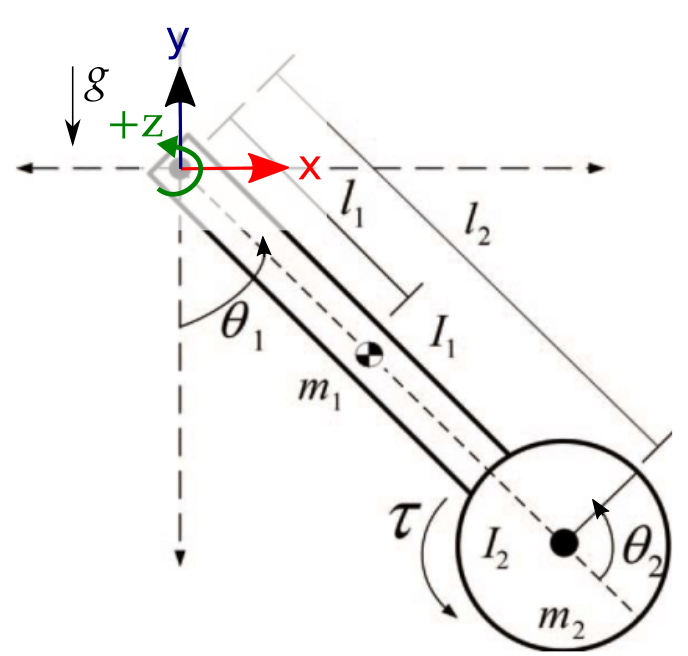
\includegraphics[width=0.5\linewidth]{images/freebody.png}
    \caption{Free body diagram}
    \label{}
\end{figure}

\subsection{Constants}
See \ref{tbl:constants}
\begin{table}[!h]
    \renewcommand{\arraystretch}{1.5}
    \caption{System Constants}
    \label{tbl:systemparameters}
    \centering
    \begin{tabular}{|c|c|}
        \hline
        Property & Measurement \\
        \hline
        $m_{stick}$ = & 115 g \\
        $m_{flywheel}$ & 546 g\\
        $m_{motor}$ & 450 g \\ % TODO: estimated
        $l_{stick} $ & 21 cm \\
        $r_{flywheel}$ & 8.5 cm \\ % TODO: estimated
        \hline
    \end{tabular}
    \label{tbl:constants}
\end{table}

\subsection{Applying LQR}

Now that we have $A$ and $B$, the matrices for our linearized dynamics of form
$f(x) = Ax + Bu$, we supply our Q and R cost functions and apply lqr. We care a
lot about the $\theta_1$, some about the $\dot\theta_1$, a bit about
$\dot\theta_2$, and not at all about $\theta_2$.  We also put a cost on the
input using $\textbf{R}$(here we closely follow the
assignment, since it turns out we will not be able to apply LQR to our physical
system).
%% ---------------------------------------------------------------------------
%% TODO ! change the inertia matrix and redo these numbers
%% ---------------------------------------------------------------------------
%% ---------------------------------------------------------------------------
\begin{align}
    Q &=
    \begin{bmatrix}
        10 & 0 & 0 & 0 \\
        0 & 1 & 0 & 0 \\
        0 & 0 & 0 & 0 \\
        0 & 0 & 0 & 0.1
    \end{bmatrix}\\
    R &= \begin{bmatrix} 0.1 \end{bmatrix}
\end{align}

Using the LQR function built into Drake, we get (rounded)

\begin{align}
    K &=
    \begin{bmatrix}
        -35 & 0 & -5 & -1 \\
    \end{bmatrix}\\
    S &=
    \begin{bmatrix}
        12 & 0 & 1  & 0. \\
        0 & 0 & 0 & 0 \\
        1 & 0 & 0. & 0. \\
        0. & 0 & 3 & 0.
    \end{bmatrix}
\end{align}

where K is our control matrix, operating on each of the four states ($q =
\theta_1, \theta_2, \dot \theta_1, \dot \theta_2$); and S is the solution of the
Ricatti equation.

% TODO: explore this S matrix further!!!
% Define what is the associated Ricatti equation

\subsection{Region of Attraction via Lyapunov}

We will briefly cover the region of attraction (RoA) analysis, which is covered
in the problem set already. For an LQR controller, which uses a linearization of
underlying nonlinear dynamics, this analysis tells us the region for which the
linearization is valid (where our LQR control can be used). 

Specifically, we will use Lyapunov analysis. Lyapunov analysis is a relaxed
optimization guarantee -- instead of guaranteeing an controller optimal for all
states will be found, we instead guarantee a controller will be able to
accomplish a given state. 

With the LQR controller, which operates as a constant matrix times the 
state error (from the desired fixed point)

\begin{align}
    u &= - K(x_{\text{measured}} - x_{\text{fixed point}})
\end{align}

We denote the error as $\bar x = x - x_{fp}$. For our Lyapunov function, we can use the cost-to-go of the LQR solution 

\begin{align}
    V_{\text{cost-to-go}} &= \bar x^T S \bar x
\end{align}

% TODO definte lyapunov function
where $S$ is as return to us by the Drake LQR solver. This S is the solution to
the Ricatti equation (a randomly fancy name for a first order quadratic
differential equation); in steady-state, this becomes an algebriac Ricatti
equation.

Note that in performing this analysis we picked a single known
reasonble Lyapunov function. Other functions are possible, which would give
slightly different regions of attraction for the same LQR controller.

% TODO: go more into this?

The value of this function, for a given state, can then be used to bound where
our linear controls will work. In our controller, we simply check the value of
$V$ for the state we are in and compare it to this bound. If we are within the
region of attraction, we use the LQR controller. Otherwise, we use the 
swing-up controller described in the following section.

\subsection{Energy-based Controller for Swingup}

% http://underactuated.csail.mit.edu/underactuated.html?chapter=acrobot
The idea behind the energy-based swingup controller is straightforward: we add
torque in the direction that the magnitude of $\theta_1$ is increasing in. We
care to increase $\theta_1$. However, we cannot directly control $\theta_1$, but
instead apply torque to control $\theta_2$. (In jargon, this is called
"non-collocated input").

For the simple pendulum, we observed 

\begin{align}
    \dot E &= u \dot \theta
\end{align}

For our system, we rederive $\dot E$ accounting for the fact that our input is
now non-collocated.

We actually desire $\dot E$ to be zero, since our $E$ will be at steady-state,
thus our energy error is directly $\dot E$. We then derive what u must be to
drive this to zero.

% TODO

In the end, in the actual sytem, a bang-bang controller was sufficient.
Additionally, as the derivation is already covered in the homework, we will not
repeat it here.

\subsection{Controllability}

This is again covered in the homework and will not be derived here.

The existence of multiple examples online would show that this system is
generally theoretically controllable, even given torque limits. 

In our case, we can also more directly consider a quick-and-dirty calcuation:
what is maximum torque produced by gravity, compared to the maximum torque our
motor can generate? Additionally, in reality the flywheel will also saturate at
some max speed of the motor, past which back EMF will limit the speed of the
flywheel. This strongly impacts the difficulty of controlling our system. 

This analyses is omitted, as the results didn't quite match reality, and likely
would need to be tailored further for the non-idealities of our physical system.

% TODO

\subsection{Is it Underactuated?}

When talking to friends about this, one of the first questions asked was
invariable "is that really an underactuated system?" especially since we do not
care about $\theta_2$.

By the definition in the textbook, 
    A control system described by equation 1 is underactuated in state (q,q˙) at
    time t if it is not able to command an arbitrary instantaneous acceleration
    in q.
With the particular caveat that the same system could be technically be fully or underactuated at different moments in time.

\section{LQR for "System on Wheels"}


For a detour (in order to demonstrate understanding of the problem set material)
we imagine sticking the whole thing on wheels and redo the same analysis,
although for sanity we run the calculations through sympy instead of by hand.


\subsection{Equations of Motion}

\noindent 1) \textbf{Write the KE of the system}. We can decompose this into the translational and
rotational components. First, let's write the x and y components of each part.
The cart is located at x = $x$ and y = 0.

\begin{align}
    \text{position\_cart} &= [x, 0] \\
    \text{position\_stick} &= [x + l_1 \sin(\theta_1), l_1 \cos(\theta_1)] \\
    \text{position\_wheel} &= [x + l_2 \sin(\theta_1), l_2 \cos(\theta_1)]
\end{align}


Asking sympy to take derivatives since it's easy to drop terms by hand,

\begin{align}
    \text{velocity\_cart} &= [\dot x, 0] \\
    \text{velocity\_stick} &= [l_1 \dot\theta_1 \cos(\theta_1) + \dot x, - l_1 \dot\theta_1 \sin(\theta_1)] \\
    \text{velocity\_wheel} &= [l_2 \dot\theta_1 \cos(\theta_1) + \dot x, -l_2 \dot\theta_1 \sin(\theta_1)]
\end{align}

Then we get

\begin{align}
    KE_{\text{translational}} &= \frac{1}{2} M \text{v\_cart}^2 + \frac{1}{2} m_1 \text{v\_stick}^2 + \frac{1}{2} m_2 \text{v\_wheel}^2
\end{align}

And as before we get the inertial kinetic energy term

\begin{align}
    KE_{\text{inertial}} &= \frac{1}{2} I_1 \dot\theta_1^2 + \frac{1}{2} I_2 (\dot\theta_1 + \dot\theta_2)^2
\end{align}


\noindent 3) Now we have the Lagrangian $L = KE - PE$ and must take the partial of the Lagrangian with
respect to each state variable, in our case $x$, $\theta_1$ and $\theta_2$.
        %-g l_1 m_1 \sin(\theta_1) - g l_2 m_2 \sin(\theta_1)
        %+ l_1^2 m_1 \dot \theta_1^2 \sin(\theta_1) \cos(\theta_1) 
        %- l_1 m_1 \dot \theta_1 (l_1 \dot \theta_1 \cos(\theta_1) + \dot x) \sin(\theta_1) 
        %+ l_2^2 m_2 \dot\theta_1^2 \sin(\theta_1) \cos(\theta_1) 
        %- l_2 m_2 \dot \theta_1 (l_2 \dot \theta_1 \cos(\theta_1) + \dotx \sin(\theta_1) \\

\begin{align*}
    \frac{\partial L}{\partial q} &=
    \begin{bmatrix}
        0 \\
        -(g m_1 l_1 + g m_2 l_2 + m_1 l_1 \dot \theta_1 \dot x + m_2 l_1 \dot \theta_1 \dot x \sin(\theta_1))\\
        0
    \end{bmatrix}
\end{align*}

\noindent 4) As an intermediate step, we calculate the partial of $L$ with
respect to $\dot q$,  $\frac{\partial L}{\partial \dot q}$.

Here we copy from sympy the three terms

\begin{lstlisting}
([[M*xdot + m1*(2*l1*t1dot*cos(t1) + 2*xdot)/2 + m2*(2*l2*t1dot*cos(t1) + 2*xdot)/2, 

1.0*I1*t1dot + 0.5*I2*(2*t1dot + 2*t2dot) + l1**2*m1*t1dot*sin(t1)**2 + l1*m1*(l1*t1dot*cos(t1) + xdot)*cos(t1) + l2**2*m2*t1dot*sin(t1)**2 + l2*m2*(l2*t1dot*cos(t1) + xdot)*cos(t1), 

0.5*I2*(2*t1dot + 2*t2dot)]]))
\end{lstlisting}


\noindent 5) Finally, we calculate the time derivative of the previous term.
Here we again note directly from sympy $\frac{d}{dt} \frac{\partial L}{\partial
\dot q_i}$ = 

\begin{lstlisting}
t1ddot*(l1*m1 + l2*m2)*cos(t1) - t1dot**2*(l1*m1 + l2*m2)*sin(t1) + xddot*(M + m1 + m2)],

1.0*I1*t1ddot + 1.0*I2*t1ddot + 1.0*I2*t2ddot + 1.0*l1**2*m1*t1ddot - 1.0*l1*m1*t1dot*xdot*sin(t1) + 1.0*l1*m1*xddot*cos(t1) + 1.0*l2**2*m2*t1ddot - 1.0*l2*m2*t1dot*xdot*sin(t1) + 1.0*l2*m2*xddot*cos(t1),

1.0*I2*(t1ddot + t2ddot)
\end{lstlisting}

\noindent 6) We set the equation equal, on the right hand side, to our input torque $\tau$.  We may then directly ask sympy to solve for $\ddot q$

\begin{lstlisting}
xddot= -(l1*m1 + l2*m2)*(0.5*g*(l1*m1 + l2*m2)*sin(2.0*t1) + t1dot**2*(I1 + l1**2*m1 + l2**2*m2)*sin(t1) + tau*cos(t1))/(I2*(M + m1 + m2) + (l1*m1 + l2*m2)**2*cos(t1)**2 - (M + m1 + m2)*(I1 + I2 + l1**2*m1 + l2**2*m2))

t1ddot= (g*(l1*m1 + l2*m2)*(M + m1 + m2)*sin(t1) + 0.5*t1dot**2*(l1*m1 + l2*m2)**2*sin(2.0*t1) + tau*(M + m1 + m2))/(I2*(M + m1 + m2) + (l1*m1 + l2*m2)**2*cos(t1)**2 - (M + m1 + m2)*(I1 + I2 + l1**2*m1 + l2**2*m2))

t2ddot= (-I2*g*(l1*m1 + l2*m2)*(M + m1 + m2)*sin(t1) - 0.5*I2*t1dot**2*(l1*m1 + l2*m2)**2*sin(2.0*t1) + tau*((l1*m1 + l2*m2)**2*cos(t1)**2 - (M + m1 + m2)*(I1 + I2 + l1**2*m1 + l2**2*m2)))/(I2*(I2*(M + m1 + m2) + (l1*m1 + l2*m2)**2*cos(t1)**2 - (M + m1 + m2)*(I1 + I2 + l1**2*m1 + l2**2*m2)))
\end{lstlisting}

\subsection{Linearization}

With the above values, we can linearize as before. Our A matrix should now be a
6x6 matrix instead of a 4x4 matrix. Solving for  $\dot x = A x + B u$

\begin{align}
    \dot x &=
    \begin{bmatrix}
        \dot x \\
        \dot \theta_1 \\
        \dot \theta_2 \\
        \ddot x \\
        \ddot \theta_1 \\
        \ddot \theta_2 \\
    \end{bmatrix},
    Ax = 
    \begin{bmatrix}
        0 & 0 & 0 & 1 & 0 & 0 \\
        0 & 0 & 0 & 0 & 1 & 0 \\
        0 & 0 & 0 & 0 & 0 & 1 \\
        (\text{see } \ddot x \text{ above}) \\
        (\text{see } \ddot \theta_1 \text{ above}) \\
        (\text{see } \ddot \theta_2  \text{ above}) \\
    \end{bmatrix} 
    \begin{bmatrix}
        x \\
        \theta_1 \\
        \theta_2 \\
        \dot x \\
        \dot \theta_1 \\
        \dot \theta_2 \\
    \end{bmatrix}
\end{align}


\subsection{LQR}

Now we can directly plug A, B, Q, and S into LQR to get out a linear controller.
This is ommitted for time reasons. The Lyapunov analysis should follow easily as
well from the problem set. The energy shaping analysis requires more
modification, but is omitted for time reasons.


%https://ocw.mit.edu/courses/mechanical-engineering/2-003sc-engineering-dynamics-fall-2011/lagrange-equations/MIT2_003SCF11_rec8notes1.pdf


%\subsection{Controllability}

%We begin by analyzing the controllability of the system. At an intuitive level,
%we see that we've added a state (the x position of the cart) without adding any
%control inputs (we can still only control the flywheel directly). We might
%expect that we can still stabilize the system, but cannot control the cart
%position while keeping the pendulum upright (at least with LQR feedback).

%To check our intuition, we check the rank of the controllability matrix, defined as



%RS-550S-18V
%https://www.harborfreight.com/18-volt-cordless-38-drilldriver-with-keyless-chuck-68239.html
%https://grabcad.com/library/rs-550s-18v-harbor-freight-900rpm-18v-cordless-drill-motor-and-gearbox-1#!


%\section{Discussion}

%\subsection{Discussion}

%1) estimate motor velocity: if we wanted to, we could do it from current

%It does seem from online that it's possible to stabilize with this estimate
%(link to youtube video)

%2) rebuild with less torque limited (maybe try this analysis again? I didn't get
%it to work above -- skip if running out of time)



%\subsection{Mechanical Lessons Learned}

%Pressfits are great! They’re used for… everything.
%Decisiveness is good – we weren’t certain about going for the better motor, which instinctually thought it’d be needed but went for it and glad we did.
%Glad we gave some consideration to clearance – bigger motor and flwheel barely fit (scrapes the staples).
%Maybe would go back to 3d printed version
%Current control


\section{Conclusion and Future Work}

In conclusion, we learned about motor control in real life, and were able to
apply several of the concepts learned in class to a real hardware system. We
encountered issues such as not being able to measure all the states, which meant
we could not use the LQR controller, but we were still able to use the energy
swing-up idea and a PD controller (which is kind of like half an LQR
controller...). Future work should include verifying robustness and region of
attraction on a physical system.

\newpage
%We got it to invert!
%In the future, LQR ... :'( 
%But for simple systems like this inverted pendulum (and not humanoids) PD is
%plenty, don't need LQR really.
%And then... stick it on wheels! -- however this version will likely be 3d
%printed...
% use section* for acknowledgment
\section*{Acknowledgments}

The authors would like to thank many people, including: on the theory side,
Elizabeth Mitten and Shane Colton for theory help, the TAs Wei Gao and Yunzhu
Li, the instructor Prof. Russ Tedrake. Motor control discussion, Bayley Wang
(and Shane). PD tuning method, Ben Katz.

%\end{thebibliography}

\bibliographystyle{IEEEtran}
\bibliography{IEEEabrv,references}
\bibdata


%\section*{ACKNOWLEDGMENT}
%\section*{Acknowledgments}

% Thanks to D. Perrin and the CSAIL community for fidicual software help
% help, B. Wang and MITERS for 3D printing, S. Colton, I. Tolkova, K. Sebesta,
% A. Pas, M. Rodruigez and N. Kirkby for paper advice.

\clearpage

\section*{APPENDIX}
\subsection{Code for Equations of Motion (flywheel pendulum)}

\lstset{basicstyle=\footnotesize\ttfamily,breaklines=true}
\begin{lstlisting}[language=Python,frame=single]  % Start your code-block


import sympy
from sympy import sin, cos, simplify, Derivative, diff
from sympy import symbols as syms
from sympy.matrices import Matrix
from sympy.utilities.lambdify import lambdastr

import time


t1, t2, t1dot, t2dot, t1ddot, t2ddot, tau = syms('t1 t2 t1dot t2dot t1ddot t2ddot tau')
m1, l1, I1, m2, l2, I2, g = syms('m1 l1 I1 m2 l2 I2 g')

p = Matrix([m1, l1, I1, m2, l2, I2, g])      # parameter vector
q = Matrix([t1, t2])

qdot = Matrix([t1dot, t2dot]) # time derivative of q
qddot = Matrix([t1ddot, t2ddot]) # time derivative of qdot
K_translat = Matrix([0.5 * m1 * (l1 * t1dot)**2 + \
    0.5 * m2 * (l2 * t1dot)**2])
K_inertial = Matrix([0.5 * I1 * t1dot**2 + \
                     0.5 * I2 * (t1dot + t2dot)**2])

P = Matrix([-1 * m1 * g * (l1 * cos(t1)) + -1 * m2 * g * (l2 * cos(t1))])
L =  K_translat + K_inertial - P

# To calculate time derivatives of a function f(q), we use:
# df(q)/dt = df(q)/dq * dq/dt = df(q)/dq * qdot


partial_L_by_partial_q = L.jacobian(Matrix([q])).T
partial_L_by_partial_qdot = L.jacobian(Matrix([qdot]))
d_inner_by_dt = partial_L_by_partial_qdot.jacobian(Matrix([q])) * qdot + \
    partial_L_by_partial_qdot.jacobian(Matrix([qdot])) * qddot

lagrange_eq = partial_L_by_partial_q - d_inner_by_dt

r = sympy.solvers.solve(simplify(lagrange_eq), Matrix([qddot]))

t1ddot = simplify(r[t1ddot])
t2ddot = simplify(r[t2ddot])

print('t1ddot= {}\n'.format(t1ddot));
print('t2ddot= {}\n'.format(t2ddot));

# --- Simply substitute, for theta = pi2,  sin pi = 1, sin theta ~= (pi - theta )

\end{lstlisting}

\subsection{Code for Swingup and Upright Controller}

The constants were determined by hand (in another (separate) program, two
potentiometers were wired up and used to tune the gains). 

Gain tuning proceeded as per Ben Katz's suggestion:
\begin{itemize}
    \item Set $K_p$ to zero. Increase $K_d$ until chattering unreasonable (where the
tiniest disturbance will cause motor to go forward and reverse rapidly). This
shows the maximum damping the system can produce.
\item  Next increase the $K_p$ until too much overshoot occurs.
\item  Profit.
\end{itemize}

\begin{lstlisting}[language=c]

// Modify for encoder-less (no motor encoder) new prototype 
// 16 May 2019

#include <Rotary.h>
#include <MegaMotoHB.h>
#include <math.h>

//https://cdn.usdigital.com/assets/datasheets/H5_datasheet.pdf?k=636931248608523021

// --------Lever Encoder--------
int val;
volatile int encoder1Pos = 0;
volatile int encoder2Pos = 0;
Rotary rMotor = Rotary(2, 3); // motor (theta2)
Rotary rStick = Rotary(A5, A4);  // stick (theta1)
int n = LOW;
/*const byte CPin = 0;  // analog input channel*/
/*int CRaw;      // raw A/D value*/
/*float CVal;    // adjusted Amps value*/

// --------Motor--------
int EnablePin = 8;
int duty;
int PWMPin = 11;  // Timer2
int PWMPin2 = 10;
MegaMotoHB motor(11, 10, 8);
int motor_output = 0; // command to motor

// --------P-Controller--------
double thetadot_deadband = 0.2;
double theta_deadband = 5;

int sample_time = 5; // 15 msec

double theta1 = 0.0; // get_from_encoder()
double theta2 = 0.0; // get_from_encoder()
double prev_theta1 = 0.0; // get_from_encoder()
double prev_theta2 = 0.0; // get_from_encoder()

double theta1dot = 0.0; // get_from_encoder()
double delta_theta1 = 0.0; // get_from_encoder()
double theta2dot = 0.0; // get_from_encoder()
double delta_theta2 = 0.0; // get_from_encoder()

double theta1_desired = 0.0;
double theta1dot_desired = 0.0;

double err_theta = 0.0;
double err_thetadot = 0.0;

int delta_motor = 0;
int prev_motor = 0;

bool theta_CW;
bool motor_CW;

unsigned long now = 0;
unsigned long time_elapsed;
unsigned long prev_time = 0;

double state[4];

double k = 4; // theta constant 
double kdot = -80; // thetadot 

void setup() {
    Serial.begin(230400);
    /*Serial.begin(9600); // for use with plotter tool */

    rMotor.begin();
    rStick.begin();
    PCICR |= (1 << PCIE2);
    PCMSK2 |= (1 << PCINT18) | (1 << PCINT19);
    PCICR |= (1 << PCIE1);
    PCMSK1 |= (1 << PCINT13) | (1 << PCINT12);
    sei();

    /*motorOn();*/
    motor.Enable();
    motor.SetStepDelay(1);
    /*setPwmFrequency(PWMPin, 8);  // change Timer2 divisor to 8 gives 3.9kHz PWM freq*/
}

void loop(){
    // -------- update time --------
    now = millis();
    time_elapsed = (now - prev_time);
    if (time_elapsed >= sample_time)
    {

    // -------- update theta --------
    // issue: prev_theta is the same as theta
    
    theta2 = getCurrentTheta2();
    theta1 = getCurrentTheta1();
    delta_theta2 = theta2 - prev_theta2;
    delta_theta1 = theta1 - prev_theta1;
    theta1dot = delta_theta1 / time_elapsed;
    theta2dot = delta_theta2 / time_elapsed;
    prev_theta2 = theta2;
    prev_theta1 = theta1;
    state[0] = theta1;
    state[1] = theta2;
    state[2] = theta1dot;
    state[3] = theta2dot;

    // -------- determine motor input --------
    /*Serial.println(motor_speed);*/

    err_theta = theta1 - theta1_desired; 
    err_thetadot = theta1dot - theta1dot_desired;
    motor_output = - ceil( k * (theta1 - theta1_desired) - kdot * (theta1dot - theta1dot_desired));
    delta_motor = motor_output - prev_motor;
    prev_motor = motor_output;
    //    Serial.print(motor_output);
    /*aprintf("\ntheta1 %f, t2 %f, t1dot %f, t2dot %f, out %d, deltath %f, cw ", */
    /*theta1, theta2, theta1dot, theta2dot, motor_output, delta_theta1);*/
    /*aprintf("\n %d %f %d %f %f ", delta_motor, theta1, motor_output, err_theta, err_thetadot);*/
    /*aprintf("\n %f %f %f %f ", theta1, err_theta, theta1dot, err_thetadot);*/
    /*aprintf("\n %f %f ", theta1dot, err_thetadot);*/
    aprintf("\n t1 %f errtheta %f, errdot %f, motor out %d, t1dot %f", theta1, err_theta, err_thetadot, motor_output, theta1dot);
    /*Serial.println(theta1);*/
    /*Serial.print(delta_motor);*/

    /*// -------- write appropriate motor input --------*/
    motor_output  = abs(constrain(motor_output, -150, 150));
    motor_output = 200;
    if (theta1 > 8) {
        if (theta1dot > 0.01) {
            motor.Rev(motor_output);
            /*motorCCW(abs(motor_output));*/
        }
        else if (theta1dot < 0.01) {
            motor.Fwd(-motor_output);
            /*motorCW(abs(motor_output));*/
        }
    }
    else if (theta1 < -8) {
        if (theta1dot > 0.01) {
            motor.Rev(motor_output);
            /*motorCCW(abs(motor_output));*/
        }
        else if (theta1dot < -0.01) {
            motor.Fwd(-motor_output);
            /*motorCW(abs(motor_output));*/
        }
        else {
            // do nothing
        }
    }
    else {
        // theta angle small; do nothing or use
        //motor.Stop();
        motorWrite(1);
    }

    // SANITY CHECK
    /*
    motor.Rev(200);
    delay(500);
    motor.Fwd(200);
    delay(500);
    motor.Stop();
    delay(500);
    */

    prev_time = now;
    }
}

// --------- Helper Functions -------

// -------- Motor Funcs --------


// Implement bang bang control on theta2 dot dot 
// -- This is PID loop to control actual motor speed to desired speed 
void motorWrite(int someValue) {

    if (someValue > 0) {
        if (theta2dot > 0 ) motor.Rev(someValue); //motor.Stop();
        else motor.Rev(someValue);
    }
    else if (someValue < 0) { // < 0
        someValue = abs(someValue);
        if (theta2dot > 0 ) motor.Fwd(someValue);
        else motor.Fwd(someValue);
    }
    else {
        //do nothing
    }
}
    
// -------- Angle Conversion --------
double getCurrentTheta1() { // calibration for stick encoder = 1250
    double val = (double(encoder1Pos) / 1250) * 360;
    val = fmod(val, 360);
    if (val > 180) {
        val = val - 360;
    }
    return val;
}

double getCurrentTheta2() {  // 500 ticks / rev, for motor encoder
    double val = (double(encoder2Pos) / 500 ) * 360;
    val = fmod(val, 360);
    if (val > 180) {
        val = val - 360;
    }
    return val;
}


// ---- Set interrupt to read encoder ----


// -------- Read encoders --------

ISR(PCINT2_vect) { // motor, on D2 and D3
    unsigned char result = rMotor.process();
    if (result == DIR_NONE) {
    }

    else if (result == DIR_CW) {
        encoder2Pos--;
    }
    else if (result == DIR_CCW) {
        encoder2Pos++;
    }
}

ISR(PCINT1_vect) { // stick, on A5 and A4
    unsigned char result = rStick.process();
    if (result == DIR_NONE) {
    }

    else if (result == DIR_CW) {
        encoder1Pos--;
        //        Serial.println(getCurrentTheta());
    }
    else if (result == DIR_CCW) {
        encoder1Pos++;
    }
}



//---- print help ---------
int aprintf(char *str, ...) {
  int i, j, count = 0;

  va_list argv;
  va_start(argv, str);
  for(i = 0, j = 0; str[i] != '\0'; i++) {
    if (str[i] == '%') {
      count++;

      Serial.write(reinterpret_cast<const uint8_t*>(str+j), i-j);

      switch (str[++i]) {
        case 'd': Serial.print(va_arg(argv, int)); // int  
          break;
        case 'l': Serial.print(va_arg(argv, long)); // long 
          break;
        case 'f': Serial.print(va_arg(argv, double)); // float
          break;
        case 'c': Serial.print((char) va_arg(argv, int)); // char
          break;
        case 's': Serial.print(va_arg(argv, char *)); // string
          break;
        case '%': Serial.print("%");
          break;
        default:;
      };

      j = i+1;
    }
  };
  va_end(argv);

  if(i > j) {
    Serial.write(reinterpret_cast<const uint8_t*>(str+j), i-j);
  }

  return count;
}


void setPwmFrequency(int pin, int divisor) {
  byte mode = 0;
  if(pin == 5 || pin == 6 || pin == 9 || pin == 10) {
    switch(divisor) {
      case 1: mode = 0x01; break;
      case 8: mode = 0x02; break;
      case 64: mode = 0x03; break;
      case 256: mode = 0x04; break;
      case 1024: mode = 0x05; break;
      default: return;
    }
    if(pin == 5 || pin == 6) {
      TCCR0B = TCCR0B & 0b11111000 | mode;
    } else {
      TCCR1B = TCCR1B & 0b11111000 | mode;
    }
  } else if(pin == 3 || pin == 11) {
    switch(divisor) {
      case 1: mode = 0x01; break;
      case 8: mode = 0x02; break;
      case 32: mode = 0x03; break;
      case 64: mode = 0x04; break;
      case 128: mode = 0x05; break;
      case 256: mode = 0x06; break;
      case 1024: mode = 0x07; break;
      default: return;
    }
    TCCR2B = TCCR2B & 0b11111000 | mode;
  }
}

\end{lstlisting}
















    %\section{Bill of Materials}

    %A list of the components of the sensor is found in \ref{tbl:bom}. %\begin{tabular}{@{}p{0.3\linewidth}p{0.48\linewidth}p{0.12\linewidth}@{}}
    %%${@{}lll@{}}
    %\begin{table}[h]
        %\caption{List of components and approximate costs}
        %\label{tbl:bom}
        %\begin{center}
            %\resizebox{0.43\textwidth}{!}{%
                %\begin{tabular}{lll}
                    %\toprule
                    %Part          & Details   & Cost  \\ \midrule
                    %Camera        & Mini Camera module, AmazonSIN: B07CHVYTGD& \$20          \\
                    %LED           & Golden DRAGON Plus White, 6000K. 124 lumens& \$2           \\
                    %4 springs     & Assorted small springs set                        & \$5           \\
                    %3D printed pieces               & PLA filament     & \$5           \\
                    %Heat-set Threaded Inserts       & Package of 50 from McMaster-Carr (use 2)          & \$1           \\
                    %Misc. Bolts   & Hex socket head      & \$1           \\
                    %Epoxy         & 5 minute             & \$5           \\
                    %\textit{3.3 V source (Arduino)} & \textit{Optional}          & \textit{\$15} \\ \bottomrule
                %\end{tabular}%
            %}
        %\end{center}
    %\end{table}



% that's all folks
\end{document}
